\documentclass[deposito, acronym, symbols]{fei}

%\usepackage{glossaries}
\usepackage{subcaption} 
\usepackage{graphicx}
\usepackage{float}
%\usepackage{units}
\usepackage[portuguese]{algorithm2e}
\usepackage{biblatex}
\usepackage{amsmath}
\usepackage{listings}
\usepackage[utf8]{inputenc}
\usepackage{chngcntr} %Faz com que o numero das notas de rodape aumente crescentemente.
\usepackage{appendix}
\counterwithout{footnote}{chapter}% "
\usepackage{siunitx}
\sisetup{output-exponent-marker=\ensuremath{\mathrm{e}}} %Escrita que precede cada entrada na lista de ilustrações.
\renewcommand{\cftfigurepresnum}{Figura }
\setlength{\cftfigurenumwidth}{5.7em}

\usepackage{titling}

%\makeglossaries
%%\newacronym[] {achpt} {ACT} {Aparecido ChupeTão}

\newacronym[longplural=Associações Brasileiras de Normas Técnicas]{abnt}{ABNT}{Associação Brasileira de Normas Técnicas}

\newacronym{ibge}{IBGE}{Instituto Brasileiro de Geografia e Estatística}

\newacronym{ashrae}{ASHRAE}{\textit{American Society of Heating, Refrigerating and Air-Conditioning Engineers}}

\newacronym{nbr}{NBR}{Norma Brasileira}

\newacronym{pmv}{PMV}{\textit{Predicted Mean Vote}}
	
\newacronym{ppd}{PPD}{\textit{Predicted Percentage of Dissatisfied}}
		
\newacronym{vgd}{VGD}{Ventilação Geral Diluidor}
		
\newacronym{vgl}{VGL}{Ventilação Local Exaustora}
		
\newacronym{cfd}{CFD}{\textit{Computational Fluid Dynamics}}
		
\newacronym{pcb}{PCB}{\textit{Printed Circuit Board}}
		
\newacronym{sms}{SMS}{\textit{Short Message Service}}
		
%\newglossaryentry{pi}{parent=greek,type=symbols,name={\ensuremath{\pi}},sort=p,description={número irracional que representa [razão entre a circunferência de qualquer círculo e seu diâmetro]}}
		


\title{TORNEAMENTO EM MATERIAL ENDURECIDO - Grupo C}
\author{ Felipe Estevão Coquito de Mello - 11.120.486-3 \\ Gabriel Mola da Silva - 11.120.255-2 \\ Netuno Trindade Torrente Rovaroto - 11.120.321-2 \\ Diurno - Vitoria Fedatto Stefaneli - 11.120.497-0}
\cidade{São Bernardo do Campo}
\instituicao{Centro Universitário FEI}

\addbibresource{Referencias.bib}
%\bibliographystyle{plain}
\bibliography{Referencias}
\graphicspath{ {Imagens/}, {Tabelas/}}

\begin{document}
\maketitle

\begin{folhaderosto}
Relatório apresentado ao departamento de Engenharia Mecânica do Centro Universitário FEI, como parte dos requisitos de avaliação da disciplina ME140 – Usinagem. Solicitado pelo Prof. Adalto de Farias.
\end{folhaderosto}

\tableofcontents
\listoffigures
\listoftables

\begin{resumo}

Usinagem é o processo de fabricação a partir do desgaste de material, na maioria das vezes esse material é um metal como aço. A usinagem em material endurecido não é diferente, porém, tem-se um metal muito duro, neste caso, normalmente com algum tipo de tratamento térmico previamente realizado. O objetivo deste relatório é analisar quais variáveis influenciam mais nas forças de usinagem e na rugosidade do material. Dito isto, foram realizados ensaios em um torno CNC, e foram verificadas as rugosidades de cada ensaio, com o auxílio de um rugosímetro. Para título de comparação os dados foram analisados, também, no software Minitab e posteriormente gerados gráficos comparativos para cada parâmetro de corte e sua influência nos esforços de corte.

\palavraschave{Usinagem. Torneamento. Material duro. Otimização.}

\end{resumo}

\chapter{Introdução}

Usinagem é o processo de fabricação a partir do desgaste de material, na maioria das vezes esse material é um metal como Aço. Sendo a usinagem de material endurecido a remoção de material de um metal com uma elevada dureza, essa dureza muitas vezes é alcançada com o material sendo submetido a um tratamento térmico para aumentar sua dureza.

Esse processo é utilizado para fabricar peças com geometrias complexas, com necessidade de alta precisão dimensional e bom acabamento superficial, que dificilmente seriam obtidas por outros métodos.

\section{Problemas e motivações para o estudo}

No meio da confecções de peças, em específico na usinagem, existe um enorme interesse na otimização dos processos, ou seja encontrar o melhor custo beneficio na produção de cada peça, porém sem comprometer o produto final para o cliente.

Neste contexto, se faz necessário o estudo de quais variáveis durante a usinagem da peça influencia diretamente na qualidade final do produto e quais variáveis influenciam para otimizar a obtenção do usinado.


\section{Objetivos do trabalho}

O objetivo desse trabalho é estudar a influencia dos parâmetros de corte, da velocidade de corte ($Vc$), do avanço ($f_n$) e da profundidade de corte ($a_p$) nos esforços em Aço endurecido, ABNT 52100, submetido ao torneamento em uma maquina CNC, assim como o estudo da variação da rugosidade da peça para diferentes parâmetros. 

\chapter{Referencial teórico}

Segundo, \textcite{farias2009analise}, Torneamento em Material é um processo de usinagem de matérias com dureza superior a 600 $HV$ (55 $HRC$), as vantagem de tal processo é destacado obtenção de medidas finais sem o uso da retificação além de diminuir os riscos de distorção durante etapas de tratamento térmico, essas características juntas diminuem o retrabalho logo diminuindo o custo de produção e melhorando a produtividade. Entretanto é necessário se atentar que por conta dessa característica as forças de cortes envolvidas nesse processo podem chegar a 80\% maior do que em matérias não endurecidos, oque influencia na escolha de ferramenta para o processo de torneamento e a vida útil da pastilha.

\section{Fatores que Influenciam a Usinagem}

Considerando o ponto de acabamento superficial segundo, \textcite{gomes2016estudo}, o avanço ($f_n$) é o parâmetro de usinagem que tem maior influência. Outro ponto que deve-se atentar na definição do parâmetro de usinagem da profundidade de corte em operações de acabamento, é que este parâmetro é diretamente relacionado ao material excedente, deixado nas operações de desbaste e também nas possíveis alterações que o componente pode sofrer durante o beneficiamento por processos de endurecimento, de tal forma que as especificações finais do produto não sejam inviabilizadas. 

Nos quesitos de Força de usinagem,no torneamento, podem ser separadas algumas componentes que influenciam mais no processo, sendo essas: Força de avanço ($F_x$), Avanço ($f_n$), Força de penetração ($F_y$), Profundidade de corte ($a_p$), Força de corte ($F_z$) e a Velocidade de corte ($Vc$).Essas componentes são os principais fatores a serem estabelecidos para a usinagem da sua peça, Figura \ref{fig:Forças_FxFyFz}

\begin{figure}[!htb]
 \centering
    \caption{Representação das forças de Torneamento}
    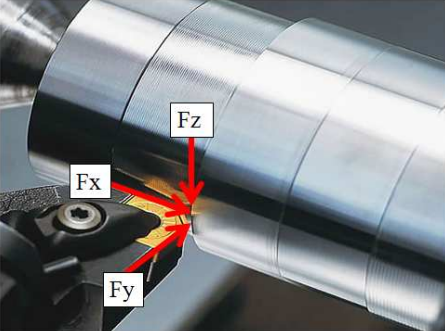
\includegraphics[width=0.5\linewidth]{Imagens/Exp02_forças_torneamento.png}
    \smallcaption{Fonte: \textcite{gomes2016estudo}}
    \label{fig:Forças_FxFyFz}
 \end{figure}

\section{Torneamento Endurecido vs Retificado}

De acordo com \textcite{gomes2016estudo}, o torneamento de material duro é um processo de fabricação que muitas vez é comparado ao processo de retificação, principalmente na areá do acabamento, pois muitas vezes é possível eliminar o processo de reificação de matérias com essa característica.

O processo de Retificação pode ser categorizado como um processo de usinagem que utiliza um rebolo abrasivo para remover material da superfície de uma peça cilíndrica com o objetivo da de obter um acabamento fino e preciso.

Uma comparação entre as características dos processos de torneamento de materiais endurecidos e retificação, foi analisada por \textcite{gomes2016estudo}, na Figura \ref{fig:Grafico_diferenças}, lembrando que os pontos mais fora do centro significam melhores resultados. O processo de torneamento demonstra vantagens como possibilitar a usinagem de geometrias complexas, é um processo mais flexível, possui alta taxa de remoção de material. O processo de retificação possui as vantagens de possui uma maior a precisão de forma e dimensão, baixos valores de rugosidade e maior confiabilidade do processo em relação ao torneamento, por conta da costeante quebra ou danificação das ferramentas. Conforme Figura \textcite{gomes2016estudo} o processo de retificação gera menores valores de tensão residual na peça usinada quando comparado ao torneamento, entretanto as tensões residuais geradas pela retificação são geralmente de tração, o que é relacionado principalmente ao efeito térmico durante o corte. Por conta dessas características muitas vezes é possível eliminar o processo de retificação para alguns matérias.

\begin{figure}[!htb]
    \centering
    \caption{Gráfico da visão qualitativa das características das operações de torneamento duro e retificação}
    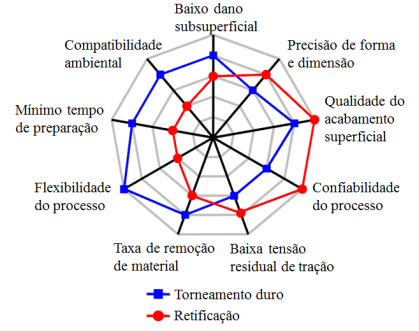
\includegraphics[width=0.65\linewidth]{Imagens/Exp02_grafico_comparado.png}
    \smallcaption{Fonte: \textcite{gomes2016estudo}}
    \label{fig:Grafico_diferenças}
 \end{figure}

\chapter{Metodologia}

Em aula o orientado disponibilizou os dados, para iniciar o planejamento dos ensaios, os dados estão disponível na Tabela \ref{tab:Variaveis}.

\begin{table}[!htb]
 \centering
    \caption{Valores designado ao grupo}
    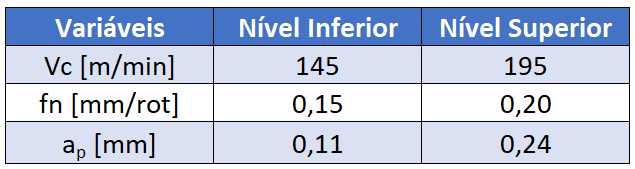
\includegraphics[width=0.65\linewidth]{Imagens/Exp02_variaveis.png}
    \smallcaption{Fonte: Autor}
    \label{tab:Variaveis}
 \end{table}

O planejamento dos ensaios foi excetuado utilizando o software Minitab, sendo composto de um Planejamento Central Composto (superfície de resposta) com três fatores ($Vc$, $f_n$, $a_p$), em dois níveis, com 4 pontos centrais e sem replicas, com randomização ativa, o resultado desse planejamento está disponível na Tabela \ref{tab:Planejamento}.

\begin{table}[!htb]
 \centering
    \caption{Planejamento gerado com utilização do Minitab}
    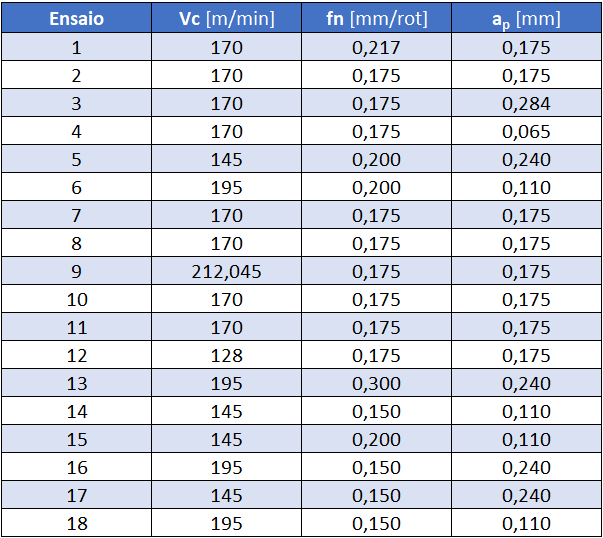
\includegraphics[width=0.85\linewidth]{Imagens/Exp02_planejamento.png}
    \smallcaption{Fonte: Autor}
    \label{tab:Planejamento}
 \end{table}

 \section{Experimento}

 O experimento foi realizado no Centro de Laboratórios Mecânicos da FEI (CLM), utilizando o Torno CNC ROMI E320, Figura \ref{fig:CNC} e a ferramenta de corte VBMT 160404-PM, Figura \ref{fig:Ferramenta} com o material de estudo sendo o Aço ABNT 52100, que possuiu um alto teor de Carbono, e sua dureza medida em Rockwell B. de 175 $HRC$.

\begin{figure}[!htp]
  \centering
  \begin{minipage}{0.4\textwidth}
    \centering
    \caption{Torno CNC}
    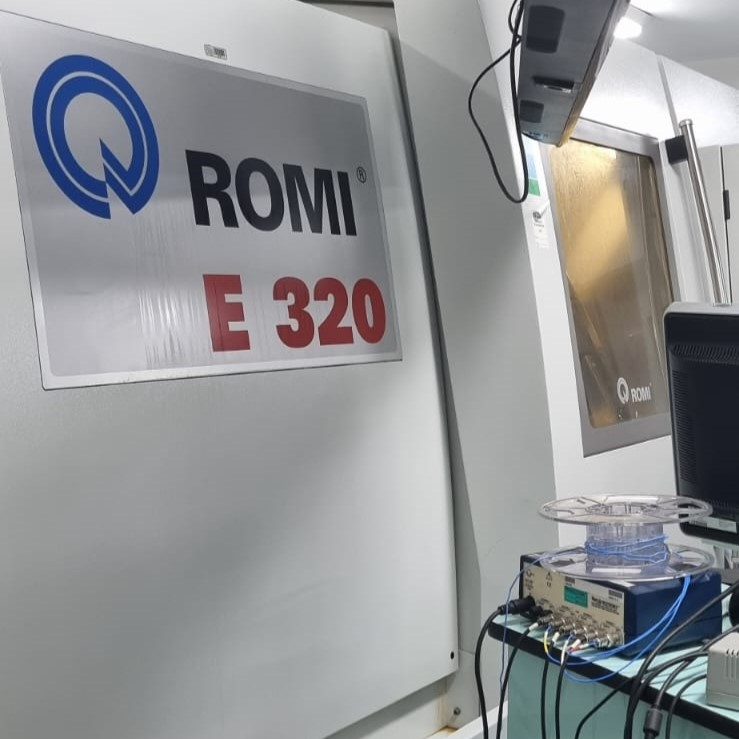
\includegraphics[width=1\linewidth]{Imagens/Exp02_CNC.jpeg}
    \smallcaption{Fonte: Autor}
    \label{fig:CNC}
  \end{minipage}
  \hfill
  \begin{minipage}{0.4\textwidth}
        \caption{Ferramenta}
    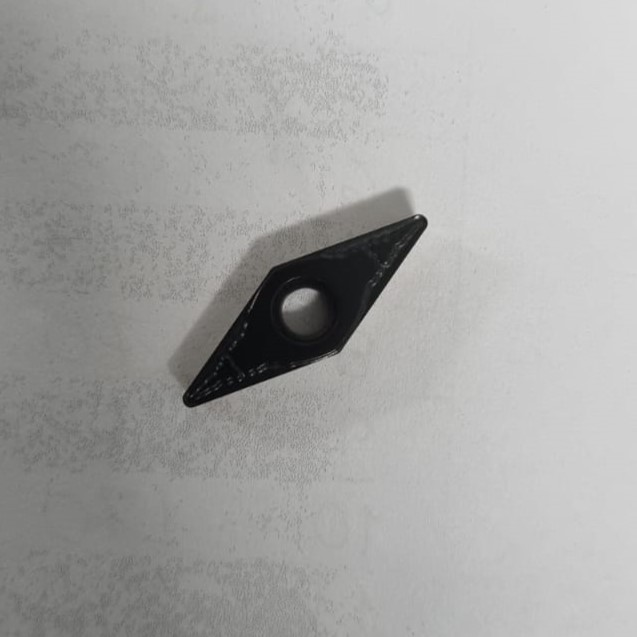
\includegraphics[width=1\linewidth]{Imagens/Exp02_ferramenta.jpeg}
    \smallcaption{Fonte: Autor}
    \label{fig:Ferramenta}
  \end{minipage}
\end{figure}

Foram feitos dois experimentos simultâneos, um com o objetivo de pegar os dados de esforço, através dos dados obtidos da medição dos Strain Gauge e outro com objetivo de colher os dados de rugosidade, através do rugosímetro.

Após a montagem da ferramenta e posicionamento da peça na placa de três castanhas, Figura \ref{fig:exp} a sequência do experimento se deu por: 

\begin{enumerate}
    \item Colocar os valores correspondeste de $n$ , $f_n$ e $a_p$ do ensaio a ser executado no torno CNC a partir da folha de Planejamento.
    \item Iniciar a operação de torneamento,
    \item Simultaneamente ao inicio da operação, começar a medição do esforço no software do computador.
    \item Finalizar a operação
    \item Salvar os dados do ensaio, Figura \ref{fig:comp}
    \item Medir a rugosidade no rugosímetro, Figura \ref{fig:rugo}, e anotar o valor indicado.
    \item Repetir para próximo ensaio.
\end{enumerate}

\begin{figure}[!htp]
    \centering
    \caption{Interior do Torno CNC}
    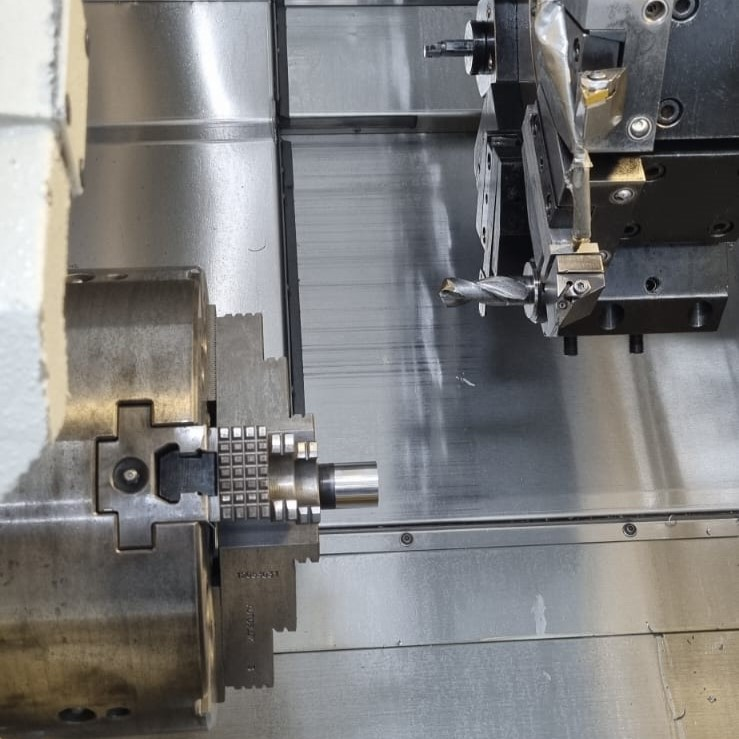
\includegraphics[width=0.6\linewidth]{Imagens/Exp02_exp.jpeg}
    \smallcaption{Fonte: Autor}
    \label{fig:exp}
\end{figure}


\begin{figure}[!htp]
  \centering
  \begin{minipage}{0.4\textwidth}
    \centering
    \caption{Computador com software de medição de esforços}
    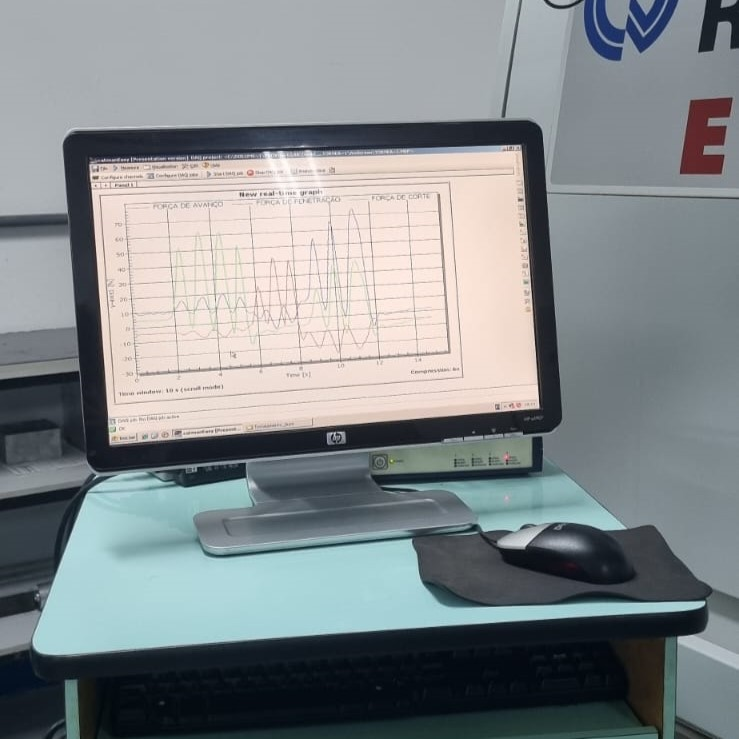
\includegraphics[width=1\linewidth]{Imagens/Exp02_computador.jpeg}
    \smallcaption{Fonte: Autor}
    \label{fig:comp}
  \end{minipage}
  \hfill
  \begin{minipage}{0.4\textwidth}
        \caption{Rugosímetro utilizado em aula}
    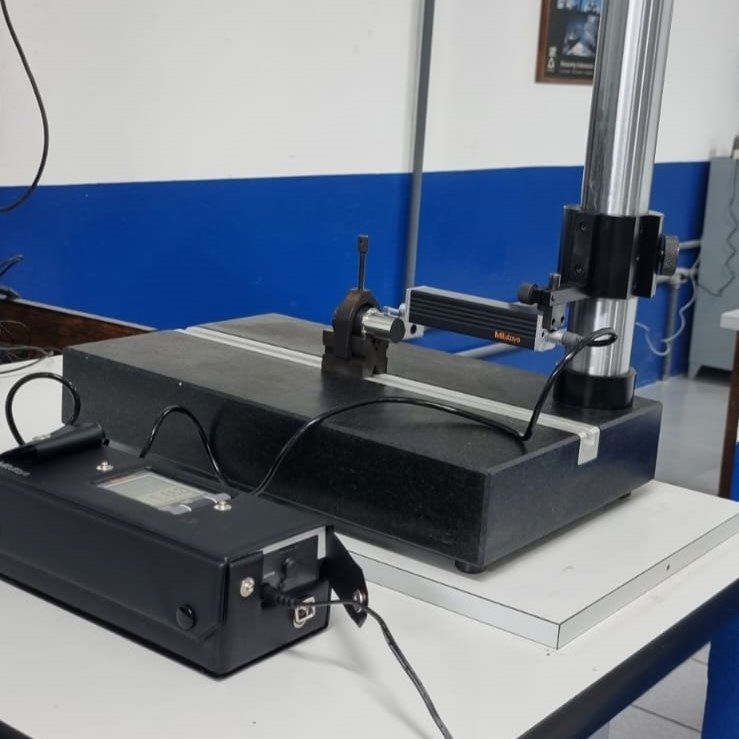
\includegraphics[width=1\linewidth]{Imagens/Exp02_rugosidade.jpeg}
    \smallcaption{Fonte: Autor}
    \label{fig:rugo}
  \end{minipage}
\end{figure}

\chapter{Resultados e Discussões}

Para realizar a etapa de discussão dos resultados, foi utilizado o software Minitab que como já citado anteriormente, nos auxiliou na análise dos dados obtidos durante o torneamento. 

\section{Esforços}

Em primeiro plano analisaremos como os parâmetros de corte, avanço ($f_n$), profundidade de corte ($a_p$), e velocidade de corte influenciam nos esforços sofridos pela ferramenta. Também será discutido e definido quais destes parâmetros mais influenciam nos esforços, sendo estes dados comprovados através de gráficos e equações gerados pelo Minitab, que serão apresentados no decorrer deste tópico. 

\subsection{Input dos dados}

Primeiramente, foram adicionados os dados da Tabela \ref{tab: minitab} ao Minitab, para que o mesmo pudesse ter as informações necessárias para realizar as comparações desejadas. Estes dados foram retirados da experiencia prática, através das células de carga. 
Ademais, foi configurado o Minitab de forma que gerasse a melhor análise possível para o caso, e indicasse os respectivos resultados desejados.

\begin{table}[!htb]
 \centering
    \caption{Planejamento gerado com utilização do Minitab}
    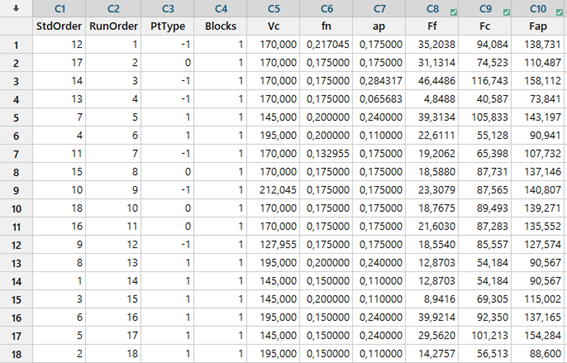
\includegraphics[width=0.85\linewidth]{Imagens/inputs minitab.png}
    \smallcaption{Fonte: Autor}
    \label{tab: minitab}
 \end{table}
 
\subsection{Response surface regression}

A primeira análise realizada é a de response surface regression, que permitiu estimar diversos resultados do experimento realizado.
Ademais, o Minitab foi configurado de forma que gerasse a melhor análise possível para o caso, e indicasse os respectivos resultados desejados.

\subsubsection{Response surface regression (Força de avanço x $f_n$, $a_p$, $Vc$)}

Realizando uma análise dos resultados da força de avanço conforme variam-se os parâmetros citados anteriormente ($f_n$, $a_p$, $Vc$), são obtidos os resultados mostrados na Tabela \ref{tab: variancias}. 

\begin{table}[!htb]
 \centering
    \caption{Analyses of Variance $F_f$}
    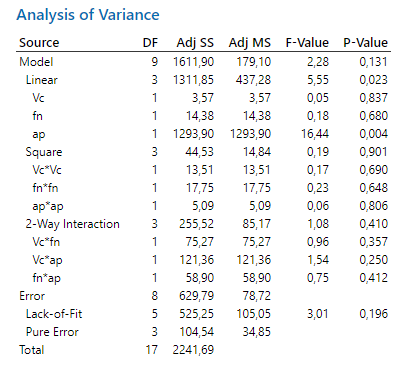
\includegraphics[width=0.85\linewidth]{Imagens/analise de variancias.png}
    \smallcaption{Fonte: Autor}
    \label{tab: variancias}
 \end{table}

Através da Tabela \ref{tab: variancias}, pode-se retirar diversas informações importantes, a primeira delas é observando a coluna de “P-Value”. Fazendo isso torna-se notório que os valores de profundidade de corte ($a_p$) são os menores valores da tabela (abaixo de 0,05, que é o valor de alpha considerado) e, portanto, tem uma confiança bem alta (de aproximadamente 95\%), tendendo então a influenciar bastante na força de avanço. 
Olhando para esta mesma tabela, porém para a coluna de “F-Value”, nota-se que o valor de profundidade de corte ($a_p$), tem o maior F-Value, o que indica que a curva deste parâmetro, que será apresentada nos próximos tópicos, terá uma grande inclinação, e, portanto, indicará que o mesmo influencia bastante no esforço analisado.

Utilizando a equação \ref{fig:eq1} pode-se estimar diferentes valores de força de avanço, para diversos valores de Velocidade de corte ($Vc$), de Avanço ($f_n$) e de profundidade de corte ($a_p$). Vale ressaltar que esta equação não fornecerá necessariamente o valor exato de força de corte, e sim uma estimativa baseada nas análises do software Minitab. 

\begin{figure}[!htp]
    \centering
    \caption{Equação da Regressão}
    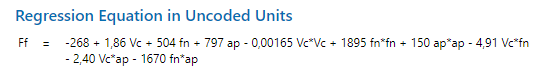
\includegraphics[width=0.7\linewidth]{Imagens/equação de regressão.png}
    \smallcaption{Fonte: Autor}
    \label{fig:eq1}
\end{figure}

Através da Figura \ref{fig:gp1}, confirma-se que o parâmetro de profundidade de corte ($a_p$) é o que mais influencia na força de avanço, isso porque ele é o único que está à direita da linha vermelha indicada no gráfico. Ou seja, os valores que estão à direita da linha vermelha influenciam mais ativamente na força de avanço, já os valores que estão à esquerda desta linha, como por exemplo a velocidade de corte e o avanço, já não influenciam tão ativamente neste esforço analisado. 
Vale ressaltar que estes resultados são considerando um alpha de 0,05, e, portanto, uma confiança de 95\%.

\begin{figure}[!htp]
    \centering
    \caption{Gráfico de Pareto}
    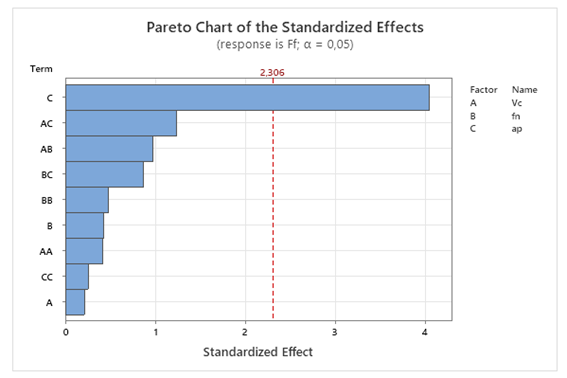
\includegraphics[width=0.7\linewidth]{Imagens/grafico pareto.png}
    \smallcaption{Fonte: Autor}
    \label{fig:gp1}
\end{figure}

Outra analise extremamente importante que pode ser retirada deste gráfico, são as possibilidades de alterações dos parâmetros, ou seja, é possível neste caso, diminuir um pouco do profundidade de corte, e aumentar os outros parâmetros, como a velocidade de corte e o avanço. 

Através da Figura \ref{fig:gr1}, é notável o quão boa ou ruim a nossa análise está, ou seja, se os resultados são verossímeis ou não. 

- Normal Probability Plot: Para ser uma boa análise, os pontos devem seguir a linha vermelha, neste caso está seguindo, portanto, indica que é uma boa análise (Verossímil).

- Versus Fit: Para ser uma boa análise, os pontos devem estar distribuídos aleatoriamente, “bagunçados”, separados uns dos outros, indicando que foi um ensaio limpo e nada influenciou negativamente. Neste caso está desta forma, portanto, é considerado uma boa análise (Verossímil).

- Histogram: Deve se assemelhar ao máximo a uma curva de distribuição normal. Neste caso está bom, mas poderia se assemelhar mais, portanto não é considerado um resultado ideal (Verossímil).

- Versus Order: Para ser considerado uma boa análise, o gráfico deve estar bagunçado e sem nenhum padrão. Neste caso analisado, está desta maneira, portanto é considerado uma boa análise (Verossímil).

\begin{figure}[!htp]
    \centering
    \caption{Gráficos Residuais de $F_f$}
    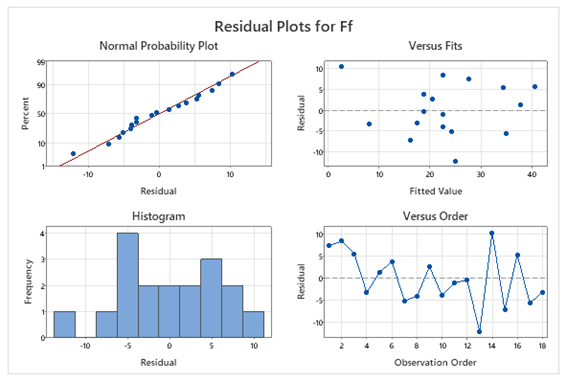
\includegraphics[width=0.7\linewidth]{Imagens/graficos residual.png}
    \smallcaption{Fonte: Autor}
    \label{fig:gr1}
\end{figure}

\subsubsection{Response surface regression (Força de corte x $f_n$, $a_p$, $Vc$)}

Será realizada, agora, uma análise semelhante à do tópico 4.1.2.1. Porém, em vez da força de avanço, será analisada a força de corte conforme se variam os parâmetros citados anteriormente ($f_n$, $a_p$, $Vc$). Em razão de as explicações seguirem a mesma linha de raciocínio anteposta e, visando evitar repetições desnecessárias, serão apresentados diretamente os resultados obtidos.

Através da Tabela \ref{tab: variancias2}, nota-se que o menor valor de P-value é para o parâmetro de profundidade de corte ($a_p$), e, portanto, indica que este é o parâmetro que tem maior influência na força de corte ($F_c$), se comparado com os outros parâmetros analisados.

\begin{table}[!htb]
 \centering
    \caption{Analyses of Variance $F_c$}
    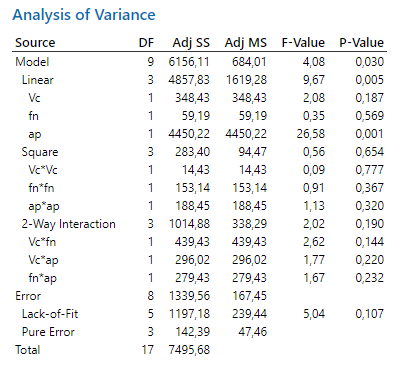
\includegraphics[width=0.85\linewidth]{Imagens/analise de variancias 2.png}
    \smallcaption{Fonte: Autor}
    \label{tab: variancias2}
 \end{table}

Observando a Figura \ref{fig:gp2} é perceptível que a profundidade de corte ($a_p$) é o único parâmetro que ultrapassa a linha vermelha, por isso pode-se dizer que é o parâmetro que mais influencia a $F_c$.


\begin{figure}
    \newpage
    \centering
    \caption{Gráficos Residuais de $F_c$}
    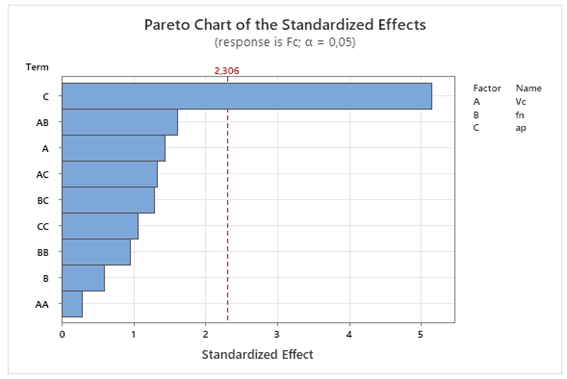
\includegraphics[width=0.65\linewidth]{Imagens/gráfico de pareto 2.png}
    \smallcaption{Fonte: Autor}
    \label{fig:gp2}
\end{figure}

A análise pelo software, de certo modo, pode ser considerada muito boa e verossímil, observando a Figura \ref{fig:gr2}.  

\begin{figure}[!htp]
    \centering
    \caption{Gráficos Residuais de $F_c$}
    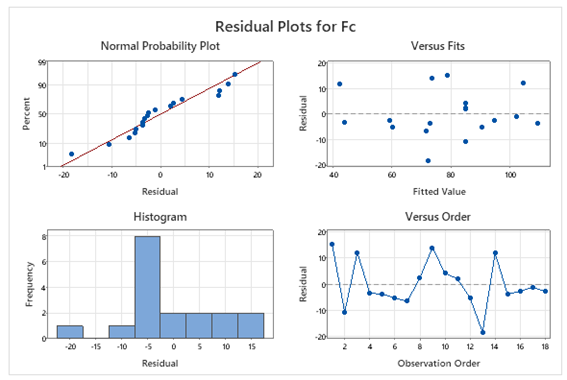
\includegraphics[width=0.65\linewidth]{Imagens/graficos residual 2.png}
    \smallcaption{Fonte: Autor}
    \label{fig:gr2}
\end{figure}

\subsubsection{Response surface regression (Força de profundidade de corte x $f_n$, $a_p$, $Vc$)}

Será realizada, agora, uma análise semelhante à do tópico 4.1.2.1. Porém, em vez da força de avanço ($F_f$), será analisada a força de profundidade de corte ($F_{ap}$) conforme variam-se os parâmetros citados anteriormente ($f_n$, $a_p$, $Vc$). Em razão de as explicações seguirem a mesma linha de raciocínio anteposta e, visando evitar repetições desnecessárias, serão apresentados diretamente os resultados obtidos.

Através da Tabela \ref{tab: variancias3}, é possível notar que o menor valor de P-value é para o parâmetro de profundidade de corte ($a_p$), e, portanto, indica que este é o parâmetro que mais influencia na força profundidade de corte ($F_{ap}$). 

\begin{table}[!htb]
 \centering
    \caption{Analyses of Variance $F_{ap}$}
    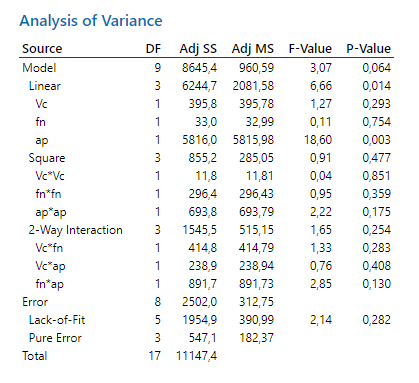
\includegraphics[width=0.6\linewidth]{Imagens/analise de variancias 3.png}
    \smallcaption{Fonte: Autor}
    \label{tab: variancias3}
 \end{table}

Confirma-se isso ao observar a Figura \ref{fig:gp3}, e notamos que a profundidade de corte ($a_p$) é o único parâmetro que ultrapassa a linha vermelha. 
  
\begin{figure}[!htp]
    \centering
    \caption{Gráficos Residuais de $F_c$}
    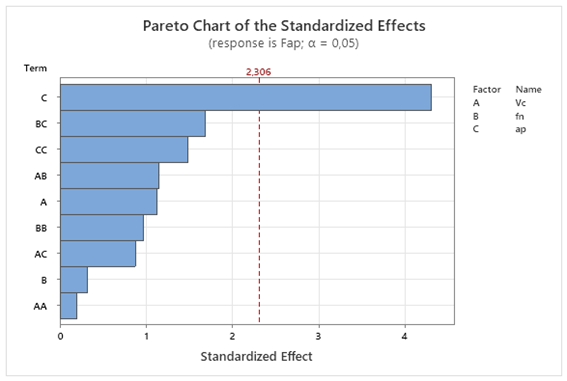
\includegraphics[width=0.6\linewidth]{Imagens/grafico de pareto 3.png}
    \smallcaption{Fonte: Autor}
    \label{fig:gp3}
\end{figure}

Vale ressaltar também que através da Figura \ref{fig:gr3}, concluiu-se que foi uma boa análise, ou seja, os resultados obtidos são bastante verossímeis.

\begin{figure}[!htp]
    \centering
    \caption{Gráficos Residuais de $F_c$}
    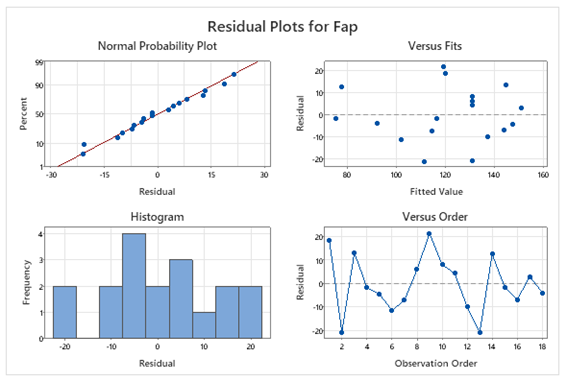
\includegraphics[width=0.6\linewidth]{Imagens/graficos residual 3.png}
    \smallcaption{Fonte: Autor}
    \label{fig:gr3}
\end{figure}

\subsection{Factorial Plots}

A segunda análise realizada durante o estudo dos esforços, nos permite confirmar através de outras métodos, os resultados obtidos no tópico 4.1.2.

\subsubsection{Factorial Plots (Força de avanço)}

A Figura \ref{fig:mff}  permite verificar e confirmar qual dos 3 parâmetros selecionados (Velocidade de corte, avanço, e profundidade de corte), mais influencia diretamente na força de avanço. Torna-se notório que a curva com um maior grau de inclinação é a curva de profundidade de corte ($a_p$), e, portanto, este é o parâmetro que mais influencia diretamente na força de profundidade de corte. 

\begin{figure}[!htp]
    \centering
    \caption{Main effects $F_f$}
    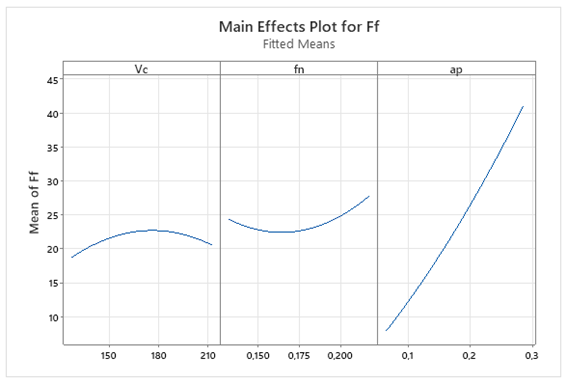
\includegraphics[width=0.6\linewidth]{Imagens/main effects ff.png}
    \smallcaption{Fonte: Autor}
    \label{fig:mff}
\end{figure}

A Figura \ref{fig:iff} permite realizar uma análise diferente das demais, afinal, ele relaciona dois diferentes parâmetros em um mesmo gráfico, demonstrando como estes dois parâmetros combinados influenciam na força de avanço. Através deste gráfico podemos notar que, mesmo que por pouco, a maior inclinação está presente quando combinamos o avanço ($f_n$) com a profundidade de corte ($a_p$), indicando que estes dois parâmetros combinados são os que mais influenciam na força de avanço. 

\begin{figure}[!htp]
    \centering
    \caption{Interection $F_f$}
    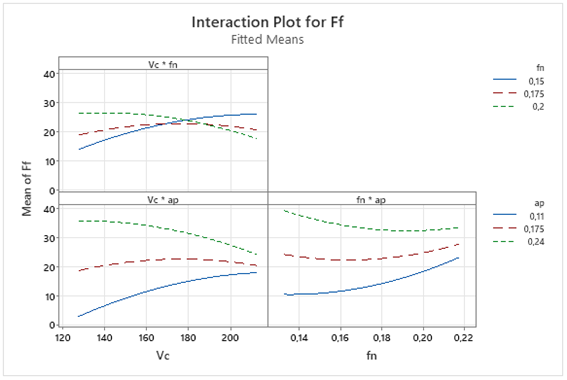
\includegraphics[width=0.6\linewidth]{Imagens/interaction ff.png}
    \smallcaption{Fonte: Autor}
    \label{fig:iff}
\end{figure}

\subsubsection{Factorial Plots (Força de corte)}

Será realizada, agora, uma análise semelhante à do tópico 4.1.3.1. Porém, em vez da força de avanço ($F_f$), analisar-se-á a força de corte ($F_c$). Em razão de as explicações seguirem a mesma linha de raciocínio anteposta e, visando evitar repetições desnecessárias, passaremos diretamente aos resultados obtidos

Através da Figura \ref{fig:mfc}, nota-se que o parâmetro com o maior grau de inclinação é o $a_p$, e, portanto, ele é o que mais influencia diretamente no força de corte. Isso confirma mais uma vez o resultado obtido no tópico 4.1.2.2.

\begin{figure}[!htp]
    \centering
    \caption{Main effects $F_c$}
    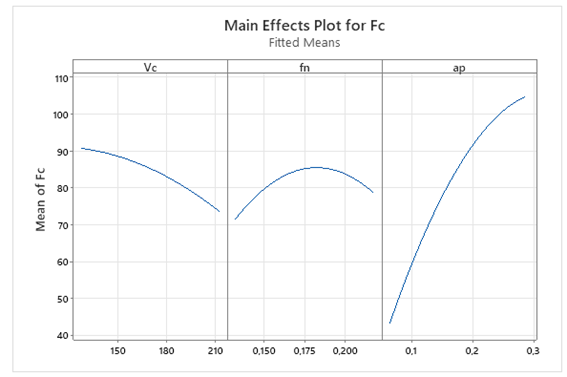
\includegraphics[width=0.6\linewidth]{Imagens/main effect fc.png}
    \smallcaption{Fonte: Autor}
    \label{fig:mfc}
\end{figure}

Através da Figura \ref{fig:ifc}, notamos que o gráfico com maior grau de inclinação é o que combina o avanço e a profundidade de corte, demonstrando que estes valores combinados são os que mais influenciam no resultado da força de corte. 

\begin{figure}[!htp]
    \centering
    \caption{Interection $F_c$}
    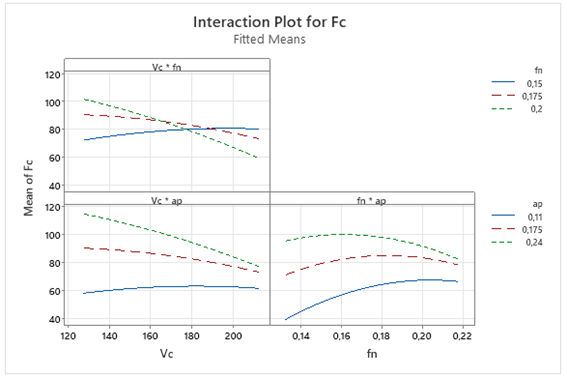
\includegraphics[width=0.6\linewidth]{Imagens/interaction fc.png}
    \smallcaption{Fonte: Autor}
    \label{fig:ifc}
\end{figure}

\subsubsection{Factorial Plots (Força de profundidade de corte)}

Será realizada, agora, uma análise semelhante à do tópico 4.1.3.1. Porém, em vez da força de avanço ($F_f$), alisar-se-á a força de profundidade de corte ($F_{ap}$). Em razão de as explicações seguirem a mesma linha de raciocínio anteposta e, visando evitar repetições desnecessárias, passaremos diretamente aos resultados obtidos

Através da Figura \ref{fig:mfap}, nota-se que o parâmetro com o maior grau de inclinação é o $a_p$, e, portanto, ele é o que mais influencia diretamente no força de corte. Isso confirma mais uma vez o resultado obtido no tópico 4.1.2.3.

\begin{figure}[!htp]
    \centering
    \caption{Main effects $F_{ap}$}
    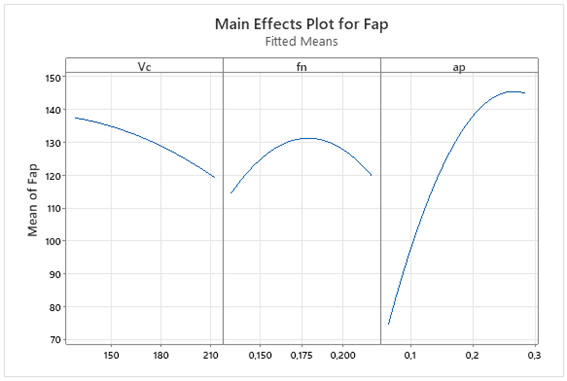
\includegraphics[width=0.6\linewidth]{Imagens/main effect fap.png}
    \smallcaption{Fonte: Autor}
    \label{fig:mfap}
\end{figure}

Através da Figura \ref{fig:ifap}, notamos que o gráfico com maior grau de inclinação é o que combina o avanço e a profundidade de corte, demonstrando que estes valores combinados são os que mais influenciam no resultado da força de corte. 

\begin{figure}[!htp]
    \centering
    \caption{Interection $F_{ap}$}
    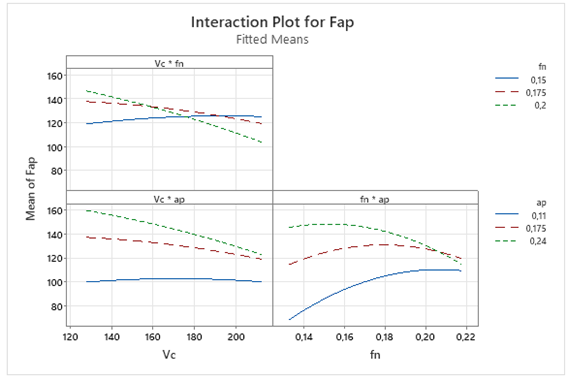
\includegraphics[width=0.6\linewidth]{Imagens/interaction fap.png}
    \smallcaption{Fonte: Autor}
    \label{fig:ifap}
\end{figure}

\subsection{Contour Plots}

Por último, foi realizado uma análise que estima os valores dos esforços desejados, conforme variamos o intervalo dos parâmetros utilizados. 

Contour Plots para Força de avanço)

Através da Figura \ref{fig:cff} podemos estimar resultados de força de avanço, conforme variamos os valores dos parâmetros dentro do range selecionado, por exemplo: 
- Para uma velocidade de corte ($Vc$) de 180, e um avanço ($f_n$) de 0,2 podemos obter um valor de força de avanço de 20 à 30. 

\begin{figure}[!htp]
    \centering
    \caption{Gráficos Contour de $F_f$}
    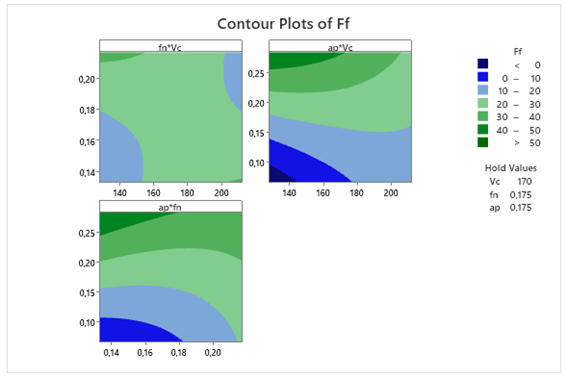
\includegraphics[width=0.6\linewidth]{Imagens/contour ff.png}
    \smallcaption{Fonte: Autor}
    \label{fig:cff}
\end{figure}

Contour Plots ( Força de corte)

Através da Figura \ref{fig:cfc}, podemos estimar resultados de força de corte, conforme variamos os valores dos parâmetros dentro do range selecionado, por exemplo: 
- Para uma velocidade de corte ($Vc$) de 180, e um avanço ($f_n$) de 0,14 podemos obter um valor de força de corte de 60 à 80. 

\begin{figure}[!htp]
    \centering
    \caption{Gráficos Contour de $F_c$}
    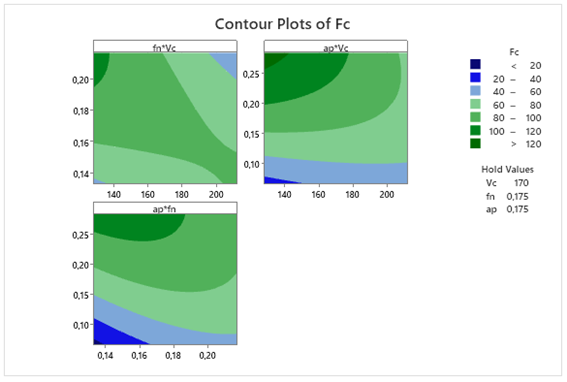
\includegraphics[width=0.6\linewidth]{Imagens/contour fc.png}
    \smallcaption{Fonte: Autor}
    \label{fig:cfc}
\end{figure}

Contour Plots (Força de profundidade de corte)

Através da Figura \ref{fig:cfap} podemos estimar resultados de força de profundidade de corte, conforme variamos os valores dos parâmetros dentro do range selecionado, por exemplo: 
- Para uma velocidade de corte ($Vc$) de 180, e um avanço ($f_n$) de 0,14 podemos obter um valor de força de profundida de corte de 100 à 125. 

\begin{figure}[!htp]
    \centering
    \caption{Gráficos Contour de $F_{ap}$}
    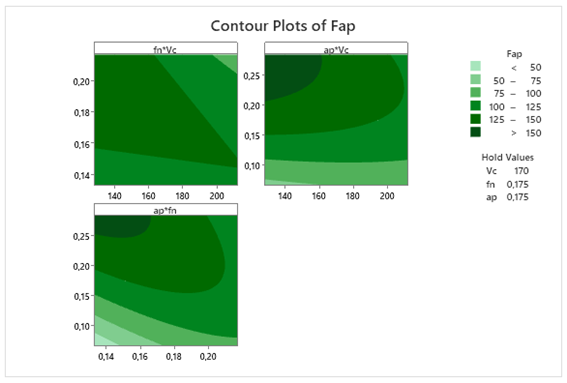
\includegraphics[width=0.6\linewidth]{Imagens/contour fap.png}
    \smallcaption{Fonte: Autor}
    \label{fig:cfap}
\end{figure}

\section{Rugosidade}

Após a apresentação e discussão dos resultados de esforços apresentados no tópico 4.1, realizaremos uma análise semelhante, porém para a rugosidade. Ou seja, será analisado como os parâmetros de anaço ($f_n$), velocidade de corte ($Vc$) e profundidade de corte ($a_p$), influenciam na Rugosidade final obtida na peça. 

\subsection{Input dos dados}

Para dar início a análise, foram adicionados os dados da Tabela 6 ao Minitab, para que ele pudesse ter as informações necessárias para realizar as comparações que desejamos. 
Vale ressaltar que estes dados foram retirados da experiencia prática, através de um equipamento medidor de rugosidades. 
Ademais, configuramos o Minitab da forma que gerasse a melhor análise possível para o nosso caso, e indicasse os respectivos resultados desejados.

\begin{table}[!htb]
 \centering
    \caption{Input dos dados de rugosidade}
    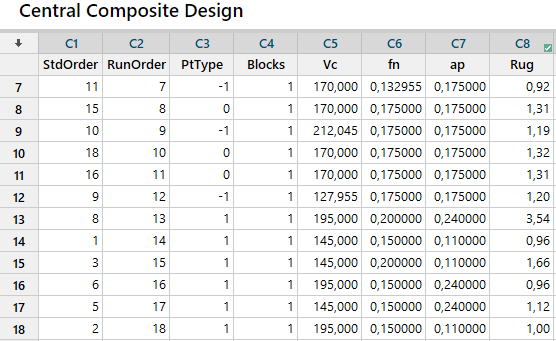
\includegraphics[width=0.6\linewidth]{Imagens/inputs minitab rug.png}
    \smallcaption{Fonte: Autor}
    \label{tab: ruginp}
 \end{table}

 \subsection{Response surface regression}
 
A primeira análise de rugosidade que foi realizada é a de response surface regression, que assim como nos esforços (Tópico 4.1.2) permite estimar diversos resultados do experimento feito.
 
Realizando uma análise dos resultados de Rugosidade conforme variamos os parâmetros citados anteriormente ($f_n$, $a_p$, $Vc$), são obtidos os seguintes resultados. 

Através da\ref{tab: rugvar1}, pode-se retirar diversas informações importantes, conforme observamos as colunas desta tabela:

- Observando a coluna de “P-Value”, torna-se notório que os valores de avanço ($f_n$) são os menores valores da tabela dentre os parâmetros utilizados (abaixo de 0,05, que é o valor de alpha considerado) e portanto tem uma confiança bem alta (de aproximadamente 95\%), tendendo então a influenciar bastante na rugosidade final da peça.

- Observando a coluna de “F-Value”, notamos que o parâmetro de avanço ($f_n$) tem o maior valor desta coluna, dentre os parâmetros inseridos, o que indica que a curva deste parâmetro, que será apresentada nos próximos tópicos, terá uma grande inclinação, e, portanto, indicará que o mesmo influencia bastante na rugosidade final da peça.

\begin{table}[!htb]
 \centering
    \caption{Input dos dados de rugosidade}
    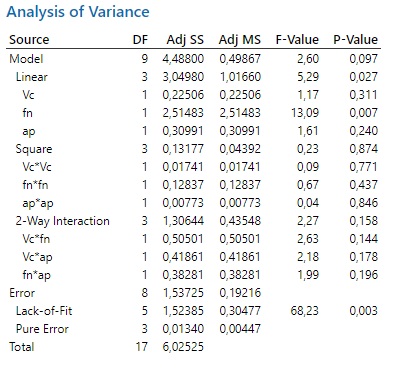
\includegraphics[width=0.6\linewidth]{Imagens/analise de variancias rug 1.png}
    \smallcaption{Fonte: Autor}
    \label{tab: rugvar1}
 \end{table}

A Figura  pode ser utilizada para estimar diferentes valores de rugosidade, para diversos valores de Velocidade de corte ($Vc$), de Avanço ($f_n$) e de profundidade de corte ($a_p$). 

Vale ressaltar que esta equação não fornecerá necessariamente o valor exato de força de corte, e sim uma estimativa baseada nas análises do software Minitab. 

\begin{figure}[!htp]
    \centering
    \caption{Equação de regressão}
    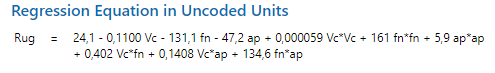
\includegraphics[width=0.6\linewidth]{Imagens/eq rug1.png}
    \smallcaption{Fonte: Autor}
    \label{fig: eqrug1}
\end{figure}

Através da Figura \ref{fig: ruggp1}, confirmamos que o parâmetro de avanço ($f_n$) é o que mais influência na rugosidade final da peça, isso porque ele é o único que está à direita da linha vermelha indicada no gráfico. 

Dessa maneira, podemos definir que os valores que estão à direita da linha vermelha influenciam mais ativamente na força de avanço, já os valores que estão à esquerda desta linha, como por exemplo a velocidade de corte e a profundidade de corte, já não influenciam tão ativamente neste esforço analisado. 

Vale ressaltar que estes resultados são considerando um Alpha de 0,05, e, portanto, uma confiança de 95%.

Outra análise importante que pode ser retirada deste gráfico, são as possibilidades de alterações dos parâmetros, ou seja, podemos neste caso, diminuir um pouco do avanço, e aumentar os outros parâmetros, como a Velocidade de corte e a profundidade de corte. 

\begin{figure}[!htp]
    \centering
    \caption{Equação de regressão}
    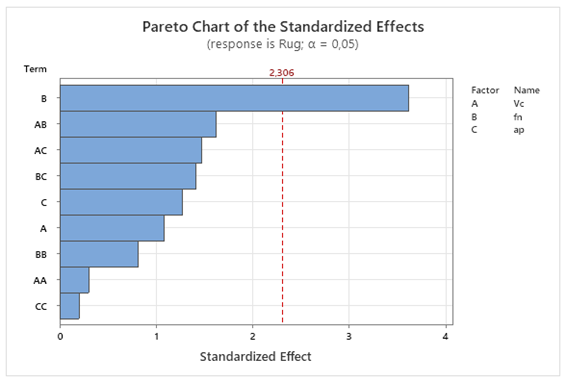
\includegraphics[width=0.6\linewidth]{Imagens/graf pareto rug1.png}
    \smallcaption{Fonte: Autor}
    \label{fig: ruggp1}
\end{figure}

Através da Figura \ref{fig: ruggr1}, podemos notar se a nossa análise está boa ou ruim, ou seja, se os resultados são verossímeis ou não. Notamos isto da seguinte forma: 

- Normal Probability Plot: Os pontos deveriam seguir a linha vermelha. Neste caso está seguindo, mas não perfeitamente, portanto, nos indica que é uma boa análise (Verossímil), mas que poderia melhor ainda mais. 

- Versus Fit: Para ser uma boa análise, os pontos devem estar distribuídos aleatoriamente, “bagunçados” e separados uns dos outros, indicando que foi um ensaio limpo e nada influenciou negativamente. Neste caso não está exatamente desta forma, portanto, é considerado uma análise razoavelmente boa (Razoavelmente verossímil).

- Histogram: Deve se assemelhar ao máximo a uma curva de distribuição normal. Neste caso está razoavelmente bom, mas poderia se assemelhar mais, portanto não é considerado um resultado ideal (Razoavelmente Verossímil).

- Versus Order: Para ser considerado uma boa análise, o gráfico deve estar bagunçado e sem nenhum padrão. Neste caso analisado, em alguns pontos existe um certo padrão, e, portanto, não esta idealmente correto, sendo considerado uma análise razoavelmente boa (Razoavelmente verossímil).

\begin{figure}[!htp]
    \centering
    \caption{Equação de regressão}
    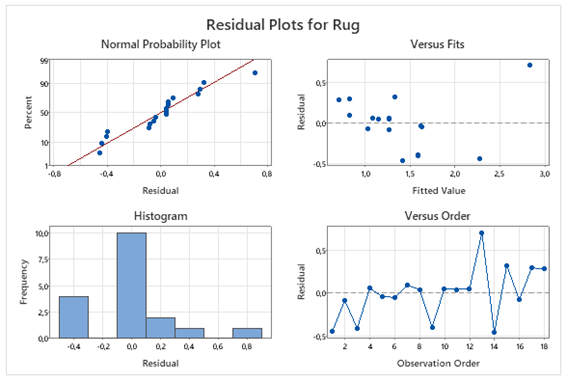
\includegraphics[width=0.6\linewidth]{Imagens/graf rsidual rug1.png}
    \smallcaption{Fonte: Autor}
    \label{fig: ruggr1}
\end{figure}

\subsubsection{Factorial Plots}

A segunda análise realizada para as rugosidades finais da peça, nos permite confirmar através de outras métodos, os resultados obtidos no tópico anterior (4.2.2).

A Figura \ref{fig:rugme2} nos permite verificar quem mais influencia diretamente na rugosidade final da peça, dentre os 3 parâmetros selecionados (Velocidade de corte, avanço, e profundidade de corte).

Sabe-se que a curva com o maior grau de inclinação, simboliza o parâmetro com maior influencia diretamente proporcional a rugosidade final da peça. E após uma simples análise torna-se notório que a curva com maior grau de inclinação é a curva de avanço, confirmando desta maneira, o resultado obtido no tópico 4.2.2, de que este parâmetro é o que mais influencia diretamente na rugosidade final da peça.

\begin{figure}[!htp]
    \centering
    \caption{Gráficos dos efeitos principais}
    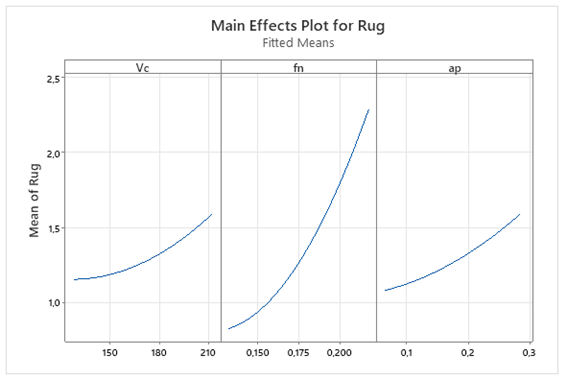
\includegraphics[width=0.6\linewidth]{Imagens/main effects rug1.png}
    \smallcaption{Fonte: Autor}
    \label{fig:rugme2}
\end{figure}

A Figura \ref{fig: rugint3} oferece uma perspectiva diferenciada em comparação com os outros gráficos, pois ele apresenta a relação entre dois parâmetros distintos em um único gráfico, revelando como a combinação desses dois parâmetros afeta a rugosidade final da peça.

Observamos a partir deste gráfico que, a maior inclinação é evidenciada quando o avanço ($f_n$) é combinado com a profundidade de corte ($a_p$), indicando que essa combinação de parâmetros exerce a maior influência sobre a rugosidade.

\begin{figure}[!htp]
    \centering
    \caption{Gráficos das intereções}
    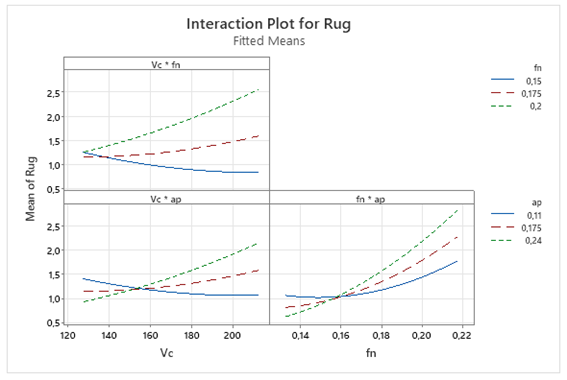
\includegraphics[width=0.6\linewidth]{Imagens/interection rug.png}
    \smallcaption{Fonte: Autor}
    \label{fig: rugint3}
\end{figure}

\subsubsection{Contour Plots}

Por último, foi realizado uma análise que estima os valores da rugosidade final da peça, conforme variamos os valores dos parâmetros utilizados, dentro dos limites escolhidos e utilizados.

Através da Figura \ref{fig: rugcont}, podemos estimar resultados de rugosidades, para 3 combinações diferentes de parâmetros (avanço e velocidade de corte, profundidade de corte e velocidade de corte e profundidade de corte e avanço). Conforme variamos os valores destes parâmetros dentro do intervalo selecionado, obtemos diferentes resultados de Rugosidade, por exemplo: 

- Para uma velocidade de corte ($Vc$) de 140, e um avanço ($f_n$) de 0,14 podemos obter um valor de rugosidade final na peça de 1,0 a 1,5. 

\begin{figure}[!htp]
    \centering
    \caption{Gráfico de contorno}
    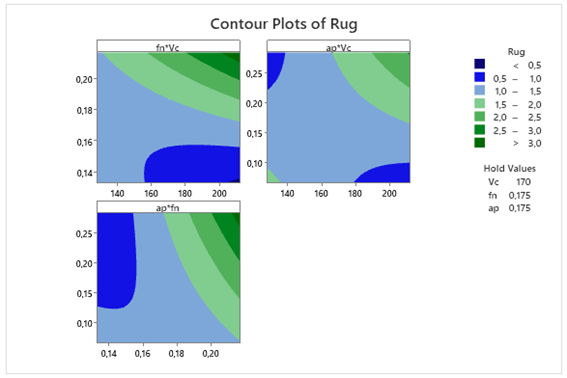
\includegraphics[width=0.6\linewidth]{Imagens/contour rug.png}
    \smallcaption{Fonte: Autor}
    \label{fig: rugcont}
\end{figure}

\chapter{Conclusões}

Conclui-se, portanto, que o parâmetro de maior influência nos esforços estudados (força de avanço, força de corte e força de profundidade de corte) é a própria profundidade de corte ($a_p$). Já para a rugosidade final da peça, torna-se notório que o parâmetro é o avanço ($f_n$). 


Em suma, após uma análise aprofundada dos dados obtidos durante a experiência empírica sobre o tema "Torneamento em material endurecido", pode-se concluir que os resultados alcançados se situam em um nível de acurácia satisfatório, embora não absoluto. Este nível de precisão ligeiramente abaixo do ideal pode ser atribuído a alguns possíveis erros ou aproximações feitas durante a aquisição dos dados. Reconhece-se que a pesquisa empírica é suscetível a variações e desafios técnicos, e, mesmo diante destes obstáculos, os resultados obtidos representam um avanço significativo no entendimento do processo de torneamento em materiais endurecidos.


\printbibliography

\end{document}